
%\documentclass{svjour3}                     % onecolumn (standard format)
%\documentclass[smallcondensed]{svjour3}     % onecolumn (ditto)
\documentclass[12pt,oneside,a4paper]{article}  

\usepackage{apacite}
\usepackage{appendix}
\usepackage{amsmath}
\usepackage{amsthm}

\usepackage{amssymb} % for approx greater than
\usepackage{caption}
\usepackage{placeins} % for \FloatBarrier
\usepackage{graphicx}
%\usepackage{subcaption}
\usepackage{longtable}
\usepackage{setspace}
\usepackage{booktabs}
\usepackage{tabularx}
\usepackage{xcolor,colortbl}
\usepackage{chngpage}
\usepackage{natbib}
\bibpunct{(}{)}{,}{a}{}{;} 
\usepackage{url}
\usepackage{nth}
\usepackage{authblk}
\usepackage[most]{tcolorbox}
\usepackage[normalem]{ulem}
\usepackage{amsfonts}
%\smartqed  
% columns for longtable
\usepackage{arydshln} % Dashed lines in matrices

\usepackage[margin=1in]{geometry}
%\doublespacing % for review
\newcommand{\absdiv}[1]{%
  \par\addvspace{.5\baselineskip}% adjust to suit
  \noindent\textbf{#1}\quad\ignorespaces
}

% line numbers to make review easier
%\usepackage{lineno}
%\linenumbers

%\usepackage{soul}% for \st{}

%%%%%%%%%%%%%%%%%%%%%%%%%%%%%%%%%%%%%%%%%%%%%%%%%%%%%%%%%%%%%%%%%%%%%%%%%%%%%%
% for section 4 math environments
\theoremstyle{definition}
\newtheorem{definition}{Definition}[section]
\newtheorem{theorem}{Theorem}[section]
\newtheorem{proposition}{Proposition}[section]
\newtheorem{corollary}{Corollary}[proposition]
\newtheorem{remark}{Remark}[section]
%

%\end{filecontents*}
%\RequirePackage{fix-cm}

% \newcommand\ackn[1]{%
%   \begingroup
%   \renewcommand\thefootnote{}\footnote{#1}%
%   \addtocounter{footnote}{-1}%
%   \endgroup
% }

% Affiliations in small font size
%\renewcommand\Affilfont{\small}

\defcitealias{HMD}{HMD 2016}

% junk for longtable caption
%\AtBeginEnvironment{longtable}{\linespread{1}\selectfont}
%\setlength{\LTcapwidth}{\linewidth}

% sort van Raalte properly
% #1: sorting key, #2: prefix for citation, #3: prefix for bibliography
%\DeclareRobustCommand{\VAN}[3]{#2} % set up for citation
\newcommand{\tc}{\quad\quad\text{,}}
\newcommand{\tp}{\quad\quad\text{.}}
%%%%%%%%%%%%%%%%%%%%%%%%%%%%%%%
\begin{document}


\title{Time spent and left of transient states in
stationary populations}

\author[1]{Tim Riffe\thanks{riffe@demogr.mpg.de}}
\author[2]{Francisco Villavicencio}
\author[3]{Nicolas Brouard}

\affil[1]{Max-Planck-Institute for Demographic Research}
\affil[2]{University of Southern Denmark}
\affil[3]{Institut National d'\'Etudes D\'emographiques}



%\authorrunning{Short form of author list} % if too long for running head

\maketitle

\vspace{-2em}
%\begin{abstract}
%\authorrunning{Short form of author list} % if too long for running head

% \institute{   Tim Riffe \at
%               Max Planck Institute for Demographic Research.
%               Konrad-Zuse-Str. 1. 18057 Rostock, Germany\\
%               \email{riffe@demogr.mpg.de}\\
%               Tel.:  +49 176 232 858 45\\
%               Fax: +49 381 2081 - 280
% \and 
% Francisco Villavicencio \at
%               Department of Public Health \& Max-Planck Odense Center on the
%               Biodemography of Aging. University of Southern Denmark, J.B. Winsl?ws Vej 9B, 
%               2nd floor DK-5000 Odense C, Denmark \\
%               \email{fvillavicencio@health.sdu.dk}
%               }
              
%\journalname{Demographic Research}
%\date{Received: date / Accepted: date}
\maketitle

\begin{abstract}
\absdiv{Background} The Brouard-Carey equality establishes equality
between the distributions of years-lived and years-left in stationary populations. 
\absdiv{Objective} This equality can be generalized to account for time
spent and time left in states within multistate stationary populations. We
provide an intuitive proof that the distribution of time spent and left in
transient states is equal in multistate stationary populations. 
\absdiv{Conclusions} We speculate that this equality may be helpful under
certain constraints to estimate the distribution of otherwise unobserved onset timing for health or other states.
%\keywords{Brouard-Carey equality \and Stationary population \and Age
%structure \and Symmetric patterns \and Multistate models}
%\subclass{91D20 \and 60K05 \and 92D25}
\end{abstract}

\section{Background}
The Brouard-Carey equality establishes that the distributions of years-lived and years-left are identical in perfectly
stationary populations
\citep{brouard1989mouvements,Vaupel2009,rao2014,villavicencioRiffeSymmetires2016}.
A perfectly stationary population is either \emph{perfectly} stationary because it is
of infinite size, because it is finite and
deterministically repeating, or as a time-invariant expectation resulting from fixed vital rates. Whether vital rates are treated as generative (traditional) or artifactual, rate schedules must be fixed and the intrinsic growth rate constant at null.

% NB: remove fertility. Define multistate stationary in a more direct a rigorous way
% as arising from fixed age-specific force of transition and mortality. No need
% to speak of fertiltiy.
Let's say that individuals in
the stationary population can obtain different states over the life course. If
birth and death rates do not vary by states, then it does not matter whether
state transition rates are fixed or not, for in the aggregate the population remains
stationary in the traditional sense. However, if vital rates depend on one's
state, transition rates must also be fixed in order for stationarity to
hold in the aggregate--- This is the situation that we entertain in the
following. Under fixed vital and state-transition rates, where vital rate
schedules differ between states, the standard set of aggregate invariant
quantities of course remains:
birth cohorts and death cohorts are of fixed and equal size. Further, the
Brouard-Carey equality still holds in the aggregate. Under these conditions,
once stationarity is achieved, the age-state structure of the stationary
population is also invariant over time, a property often exploited by Markov
models where the goal is to estimate state expectancies or similar. As a
consequence of fixed transition and vital rate schedules, the distribution of state-specific tenures for individuals entering a state at a given age is also a fixed attribute: These are mereley aggregations over individuals, and the probability of any particular life course trajectory is also fixed.

This setup is not entirely contrived, for it corresponds with the assumptions of
common multistate markov models, often used to calculate state expectancies.
In the present, however, we are not bound to memoryless transition probabilities.
Instead, we simply require the consequence of (or the expectation of) invariant
age-state structure and invariant conditional age-state tenure distributions, which may result from
either memoryless transitions, or from arbitrarily linked
dependencies.
It is the fact of fixed age-state flows and structure on which we base the following observations.
In essence, the population consists in set of lives that is a fixed distribution of lifecourse
trajectories, each consisting in a sequence of discrete state-specific
durations. This set could be of infinite size (but discrete time intervals), in
which case the fraction of births destined to live a given trajectory is fixed,
or it could exist as a fixed occurrence probability (the product of
transition probabilities required to live said trajectory). 

Under fixed vital and transition rates, and zero growth, we introduce a new
theorem, which is a more general version of the Brouard-Carey equality.
Namely, if there is some state $s$ in the population, a
randomly drawn individual from state $s$ has equal probabilities of having
entered $s$ $x$ years ago and exiting $s$ in $x$ years. This proposition
might not be intuitive at first glance, so we prove it, and then speculate
as to how this equality may be put to good use. 

\section{An intuitive proof of transient symmetry}
\FloatBarrier

% NB: change to language of x+delta x, or change to census at time t
% the probability of being < x years in state (or state 0-x years).
% same as remaining in state for at most another x years. Or something like this.
% discretize the theorem. 
\begin{theorem}
\label{th}
Given a stationary population at exact time $t$ and fixed state-transition
rates, the probability that a randomly selected individual is in state $s$ and has been in $s$ continuously for the past $x$ years
is equal to the probability of being in state $s$ and remaining in $s$ for exactly $x$ more years.
\end{theorem}

We provide two proofs of theorem~\ref{th}. The first is built from individual life courses in the stationary population (or the fixed probability thereof). The second follows the Lexis aggregate approach of \citet{villavicencioRiffeSymmetires2016}.

\begin{proof}
The proof of this statement follows five intuitive steps, built up from
the notion of a lifeline identifying the states experienced over a potential
life course.
\begin{enumerate}
\item{} A duration can be represented as a line segment, potentially a
subset of a life-line. Points along a single within-person duration can be
sampled over time in arbitrarily fine and regular time steps, $\delta$. Each
time step can then be used to bisect the segment, collecting two sets of
values: 1) time spent in the state prior to the sample point, and 2) time
left until exiting the state.
If observations are evenly spaced, and values are truncated to the nearest
$\delta$, by way of complements these two sets will consist of the same values.

If the duration of the $i^{th}$ individual is called $d^i$, the age of entry
is $a_L^i$ and the age of exit is $a_R^i$, such that $d^i = a_R^i -
a_L^i$. The set of time-spent values, $A^i$ is defined as:
\begin{align}
\label{eq:Ai}
A^i &= \left\{ \delta \cdot k ~| ~k \in \mathbb{Z}^+~, ~0 \le k \le
\left\lfloor \frac{d_i}{\delta}\right\rfloor \right\} \tc \intertext{where
$\lfloor \ldots\rfloor $ denotes truncation to the lower integer bound. The
set of time left values, $T^i$ is also:}
\label{eq:Ti}
T^i &= \left\{ \delta \cdot k ~| ~k \in \mathbb{Z}^+~, ~\left\lfloor
\frac{d_i}{\delta}\right\rfloor \ge k \ge 0\right\} \tp
\end{align}
\textcolor{red}{Note, need to choose $\mathbb{Z}^+ or \mathbb{N}$. Practically
identical. I lean toward Z because negatives have meaning, we're just not
considering them.} Figure~\ref{fig:lifeline1} illustrates the construction of
$A^i$ and $T^i$ in expressions~\eqref{eq:Ai} and \eqref{eq:Ti}. The central cut-point moves along the duration from the time of entry until the time of exit, creating two
lists of values.

\begin{figure}
\centering
\caption{A lifeline of individual $i$ showing the construction of the sets $A^i$
and $T^i$.\textcolor{red}{need to label $a_R^i$, $a_L^i$.}}
\label{fig:lifeline1}
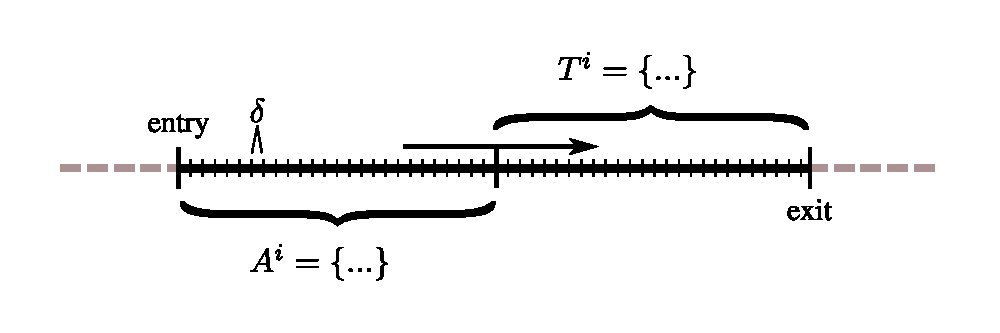
\includegraphics[scale=.8]{Figures/lifeline1.pdf}
\end{figure}

\FloatBarrier
\item{} If this exact lifecourse is replicated every $\delta$ time step (the
same spacing as our observation spacing in figure~\ref{fig:lifeline1}) in a
Lexis space, we end up with a set of identically aligned and identically long segments placed side-by-side, spaced apart by $\delta$.
This potentially large set of segments may be imagined as a plane, although this
would only hold in the limit.
One could in this setting take a census at a single point in time, collecting a set of
time spent and time left values, each from a repeated lifecourse in
sequence.
It is clear that the two sets observed at a single time point but drawn from the population of
perfect clones, will be identical to the first two sets that were observed of
a single duration over its entire length, if the same $\delta$-truncation operation is followed.

Figure~\ref{fig:clones} illustrates this notion with uniformly-spaced lifelines
in a Lexis configuration. The vertical line indicates a hypothetical census at time $t$ of
the population of this cloned individual. At time $t$, the blue-highlighted segments indicate
the set of time-spent values in $A^i$, and red-highlighted segments are the
time-left elements of $T^i$. 

 \begin{figure}[h!]
\centering
\caption{The $i^th$ lifecourse is repeated in $\delta$ time steps. A
census with followup now constructs the sets $A^i$ and $T^i$ with values
identical to the within-individual sets.\textcolor{red}{need to label $a_R^i$,
$a_L^i$,etc.}}
\label{fig:clones}
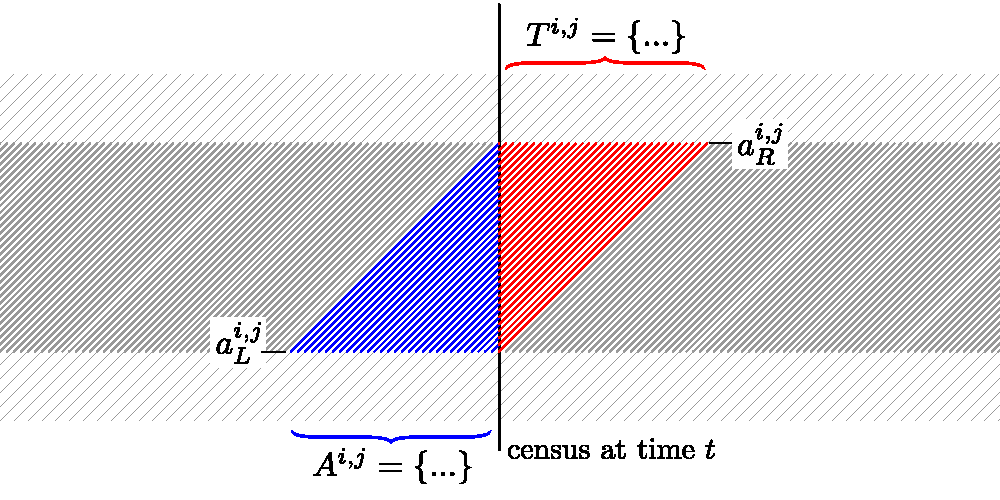
\includegraphics[scale=.8]{Figures/lifelinerepeated.pdf}
\end{figure}

Formally, sets $A^i$ and $T^i$ consist of the same values as the previous, but
coming from individuals born in a uniform series from between $t-a_R^i$ years
ago until as recently as $t-a_L^i$ years ago. This demonstrates both
period-cohort equality and time spent-left equality. The blue and red triangles in
Figure~\ref{fig:clones} are simple rotations of one another.

\FloatBarrier
\item{} Assume we have a second individual from the same birth cohort as
individual $i$ that enters the same state as the first, but at a different time
and for a different total duration. We could demonstrate time spent and time left equality in the same
way for this individual, by sampling in $\delta$ time steps. Since
this individual has a different life course timing than the first individual, their
sets of time-spent, $A^2$, and time left $T^2$ will be distinct. $A^1$ and $T^1$ range from 0 to $d^1$, whereas $A^2$ and $T^2$
range from 0 to $d^2$. However, their concatenations are identical:

\begin{equation}
\label{eq:unioneq}
\{A^1 , A^2\} = \{T^1 , T^2\}
\end{equation}

\item{} If the second individual is also perfectly cloned in $\delta$ time
steps as in step 2, then our census at a single point in time also
yields identical sets of time spent and time left values, $A^2$ and $T^2$. Also
from this census, the concatenation of the first and second time-spent sets and the concatenation of the first and second time-left sets
are guaranteed to be identical, as in equation \eqref{eq:unioneq}. 

\item{} By induction we can keep adding durations in this state, infinitely if we
please, and the collection of all resultant time-spent sets and the collection
of time-left sets will continue being identical. Therefore the probability of selecting a particular value from the time-spent set is identical
to the probability of selecting the same value from the time-left set. 
\end{enumerate}
\end{proof}

Our point of departure was that of a perfectly stationary population with
identically distributed lifelines that aggregate to a fixed age-state structure,
and this is also the result that we arrive at by induction in the final step of
the proof. In this strict environment it is therefore the case that our theorem
holds. A more rigorous proof would allow $\delta$ to decrease to 0 in the
limit. The present approach does not allow this because probability statements
would no longer hold. We may require a population of infinite size in order to
make the jump from a fixed age-state structure to an invariant set of lifelines,
where each lifeline is itself an invariant sequence of states. 

\section{Discussion}
The approach from this proof is equally valid to prove the
original statement of the Brouard-Carey equality (where the state is ``alive''),
but it is more general.
The statement and proof is flexible enough to hold for irreversible and reversible
states. It also applies to repeatable states, whether time spent in the
state is kept in cumulative fashion over spells, or whether the clock resets to
zero on each entry into the state. The equality may also be conditionable in
curious ways: for example, the distribution of time-spent in a state conditional
on having entered at age $a$ must also be equal to the distribution of time-left in
the state, conditional on having entered at age $a$. Likewise, one may condition
statements on exit age. One may also arbitrarily merge states, and the equality
still holds within the newly merged state.

At first glance, this equality is probably less intuitive than the
original Brouard-Carey equality, because state entry is not necessarily aligned
on age zero. It is less visible in commonly-produced plots because plots of
stacked sequences look chaotic, often even if clustered or sorted. It might
be tempting to think that due to state-varying vital rates, the equality simply ought not hold.
However, the basis of the proof is the observation that if each individual
duration is symmetrical by complements, then so are aggregations of
durations, irrespective of alignment. Since each cohort in a perfectly
stationary population of infinite size is an identical copy of the previous,
census-like cross-sections are also equally-composed.

\section{Potential applications}
Empirical applications of the presently-described transient tenure equality may
be easy to conjure up. For example, imagine a hypothetical health state that
shows no noticeable symptoms, but that is medically measurable. One
may take a census with regular follow-ups, until eventually the state is exited
by each individual, whether by absorption into death or entry into another
state. Then, if the assumption of stationarity is acceptable, one may be able to
say something about onset timing in the aggregate, itself unobserved. %We think
%that the present equality will come as good news to researchers in similar
%settings.

\section{Simulation}
[section commented out until exercise more completely designed]
% The reader may wish to have a sense of how well this equality holds up under
% various violations of our assumptions. The assumption of invariant transitions
% is trickier to handle than that of finite populations with stochasticity. We
% conduct a simple markov chain simulation to
% produce random populations of different sizes derived from the same
% set of stationary transition probabilities. Our transition rates come
% from a published study of working life expectancy in older ages in the USA
% \citep{Dudel2017}, and refer to US black females around the year 1994. The transition matrix includes
% single ages 50-100, with lifetable closeout at age 100. Transient states include
% employed, unemployed, inactive, and retired. We generate random sequences of
% trajectories using the \texttt{rmarkovchain} function of the
% \texttt{markovchain} \texttt{R} package \citep{spedicato2017}.
% 
% For simplicity, all trajectories begin in a state of employment at age 50. We
% generate 1000, 10000, and 100000 individual trajectories. Out of these we
% sample observations of inactivity a total of 100, 1000, and 10000 times,
% respectively with replacement. We assume that the time of
% observation is half way through the year, but that spells begin on January 1 and
% end on December 31. For each observation of inactivity we measure the time spent
% in the spell up to the point of observation, and the time left until exiting the
% spell. These values are then tabulated for each simulation to produce
% distributions to compare. The theorem states that the distributions of time
% spent and left in this procedure should be asymptotically identical, but we have
% induced noise with the simulation, and we should be able to see distributions
% converge as simulated population and draw sizes increase.
% 
% 


\section{Conclusion}
Stationary populations are more symmetrical with respect to time lived and
spent than has been previously described. We have given an intuitive proof that
the distribution of time spent and left is equal within states in
stationary populations. We do not presume that this relationship will be immediately able to answer pressing questions, but we
hope that it may inspire new approaches in empirical measurements. We think
that that researchers working with left-censored or truncated data or
any kind of multistate models should be generally aware of this equality in case
it may come in handy as a heuristic.

The relationship between years lived
and left established by the Brouard-Carey equality is itself amenable to non-zero growth rates \citep{riffe2015renewal}.
We speculate that the transient tenure equality we describe here may also be tractable in stable
populations, but we have not investigated this possibility in detail. Future
research, potentially more sophisticated simulations, should establish the
impact of departures from stationarity and establish the fuzzy bounds of
usability for this relationship.



%\bibliographystyle{chicago}
\bibliographystyle{spbasic}
\bibliography{references}  
\end{document}
